\documentclass{article}
\usepackage{amsmath}
\usepackage{amssymb}
\usepackage{amsthm}
\usepackage[english]{babel}
\usepackage{graphicx}
\usepackage{natbib}
\usepackage{authblk}
\usepackage{pdflscape}


\title{OneD: increasing reproducibility of Hi-C Samples with
abnormal karyotypes}

\author[1,2,*]{Enrique Vidal}
\author[1,2]{Fran\c{c}ois le Dily}
\author[1,2]{Javier Quilez}
\author[1,2]{Ralph Stadhouders}
\author[1,2]{Yasmina Cuartero}
\author[1,2]{Thomas Graf}
\author[1,2,3,4]{Marc A.  Mart\'i-Renom}
\author[1,2]{Miguel Beato}
\author[1,2]{Guillaume J. Filion}
\affil[1]{Gene Regulation, Stem Cells and Cancer Program, Centre for
Genomic Regulation (CRG), The Barcelona Institute of Science and
Technology (BIST), Dr. Aiguader 88, 08003, Barcelona, Spain}
\affil[2]{Universitat Pompeu Fabra (UPF), Barcelona, Spain}
\affil[3]{CNAG-CRG, Centre for Genomic Regulation (CRG), Barcelona
Institute of Science and Technology (BIST), Baldiri i Reixac 4, 08028
Barcelona, Spain}
\affil[4]{ICREA, Pg. Lluís Companys 23, 08010 Barcelona, Spain}
\affil[*]{\textbf{Contact:} enrique.vidal@crg.eu}

\begin{document}

\maketitle

\begin{abstract}
The three-dimensional conformation of genomes is an
essential component of their biological activity. The advent of the Hi-C
technology enabled an unprecedented progress in our understanding of
genome structures. However, Hi-C is subject to systematic biases that can
compromise downstream analyses. Several strategies have been proposed to
remove those biases, but the issue of abnormal karyotypes received little
attention. Many experiments are performed in cancer cell lines, which
typically harbor large-scale copy number variations that create visible
defects on the raw Hi-C maps. The consequences of these widespread
artifacts on the normalized maps are mostly unexplored.
We observed that current normalization methods are not robust to the
presence of large-scale copy number variations, potentially obscuring
biological differences and enhancing batch effects. To address this issue,
we developed an alternative approach designed to take into account
chromosomal abnormalities. The method, called \textit{OneD}, increases
reproducibility among replicates of Hi-C samples with abnormal karyotype,
outperforming previous methods significantly. On normal karyotypes,
\textit{OneD} fared equally well as state-of-the-art methods, making it a
safe choice for Hi-C normalization.  \textit{OneD} is fast and scales well
in terms of computing resources for resolutions up to 1 kbp.
\textit{OneD} is implemented as an R package
available at http://www.github.com/qenvio/dryhic.
\end{abstract}




%% --------------- Introduction --------------- %%

\section{Introduction}

One of the crown achievements of modern biology was to realize that
genomes have an underlying three-dimensional structure contributing to
their activity \citep{rowley2016three, dekker20163d, pezic2017more}. In
mammals, this organization plays a key role in guiding enhancer-promoter
contacts \citep{de2013topology}, in V(D)J recombination
\citep{choi2014ctcf} and in X chromosome inactivation \citep{galupa2015x}.
A significant breakthrough towards this insight was the development of
the high throughput chromosomal conformation capture technology (Hi-C),
assaying chromosomal contacts at a genome-wide scale
\citep{lieberman2009comprehensive}. Nowadays, exploring the spatial
organization of chromatin has become a priority in many fields and Hi-C
has become part of the standard molecular biology toolbox
\citep{dekker2013exploring}.

Contrary to the precursor technologies 3C, 4C and 5C
\citep{dekker2002capturing, simonis2006nuclear,
dostie2006chromosome,de2012decade}, Hi-C interrogates all possible
pairwise interactions between restriction fragments. However, this does
not guarantee that the method has no bias.  On the contrary, local genome
features such as the G+C content, the availability of restriction enzyme
sites and the mappability of the sequencing reads have been shown to
impact the results \citep{yaffe2011probabilistic}, in addition to general
experimental biases such as batch effects. It is thus important to
normalize Hi-C data in order to remove biases and artifacts, so that they
are not confused with biological signal.

Several methods have been proposed to remove biases in Hi-C experiments
\citep{schmitt2016genome}. The first strategy is to model biases
explicitly from a defined set of local genomic features, such as the G+C
content. This approach is used in the method of
\cite{yaffe2011probabilistic} and in Hicnorm by \cite{hu2012hicnorm}. The
second strategy is to implicitly correct unknown biases by enforcing some
regularity condition on the data. This approach is used in the
Iterative Correction and Eigenvector decomposition method (\textit{ICE})
of \cite{imakaev2012iterative}, whereby the total amount of contacts of
every bin is imposed to be the same. \textit{ICE} is currently the most
popular method, due in part to its speed.

Neither of these strategies were designed for cell types with karyotypic
aberrations, most common in cancer. Yet, Hi-C is very sensitive to
aneuploidy, copy number variations and translocations.  Actually, these
aberrations have so much influence on the outcome that they can be used as
signatureto re-assemble the target genome \citep{korbel2013genome}. An
additional complication is that karyotypic aberrations are not
experimental biases, so it is unclear whether they should be corrected at
all or be considered part of the biological signal.

So far, the only attempt to address the issue was the chromosome-adjusted
Iterative Correction Bias method (\textit{caICB}) of
\cite{wu2016computational}. However, \textit{caICB} applies a uniform
chromosome-wide copy number correction, effectively excluding the numerous
cases of partial aneuploidy and regional copy number variations.

Here we propose \textit{OneD}, a method to correct local chromosomal
abnormalities in Hi-C experiments. \textit{OneD} explicitly models the
contribution of known biases via a generalized additive model. The
normalized data is more reproducible between replicates and across
different protocols. Importantly, \textit{OneD} is also efficient when
cells have a normal karyotype, where it performs as well as the best
normalization methods. Finally, the implementation is as fast as
\textit{ICE} and it scales up to 1~kbp resolution with reasonable
computing resources.

%\enlargethispage{12pt}


\section{Methods}

\subsection{Model}
\label{sec:model}

The most common representation of Hi-C data is a contact matrix, obtained
by slicing the genome in $n$ consecutive bins of fixed size (the
resolution) and computing the number of contacts between each pair of
bins. The values are stored in the cells of the contact matrix ($x_{ij}$),
quantifying the interaction between the two loci at positions $i$ and
$j$.

Our approach is to model the tally of contacts for each bin, thus reducing
the matrix to a one dimension score (hence the name \textit{OneD}). We
assume that the total number of contacts per bin ($t_{i}$) can be
approximated by a negative binomial distribution. This choice is sensible
because the amount of contacts is a discrete variable and because the
negative binomial distribution allows for overdispersion. We further
assume that the explicit sources of bias have independent contributions to
the mean of the distribution for a given bin ($\lambda_i$).

Given that this relationship might not be linear (see for instance
Figure~\ref{fig:totals}A), we allowed a smooth representation
using thin plate penalized regression splines \citep{wood2003thin} in a
generalized additive model \citep{wood2011fast}. The model can be
parametrized as

\begin{align*}
t_i = \sum_j^n{x_{ij}} &\sim  NB(\lambda_i, \theta) \\
\log(\lambda_i) &\propto \sum_{k}{f_k(z_k)}
\end{align*}

\noindent
where $x_{ij}$ is the raw number of contacts between bins $i$ and $j$, and
$z_k$ is the additive bias of genomic feature $k$. The smooth functions
$\{f_k(\cdot)\}$ are estimated jointly with the negative binomial
dispersion parameter $\theta$ using the \texttt{mgcv} package
\citep{wood2011fast} of the R software \citep{coreteam2014r}.

Once the parameters of the model are determined, the estimated means
$\{\lambda_i\}$ are rescaled to obtain a correction vector
$\{\lambda_i'\}$ that can be used to compute the corrected counts
($\hat{x}_{ij}$).

\begin{align}
\notag
\lambda_i' &= \frac{\lambda_i}{\sum_j^n{\lambda_j}/n} \\
\label{eq:xhat}
\hat{x}_{ij} &= \frac{x_{ij}}{\sqrt{\lambda_i'\lambda_j'}}
\end{align}

In line with previous methods
\citep{yaffe2011probabilistic,hu2012hicnorm}, the default features
used to fit the model are the local G+C content, the read mappability and
the content and number of restriction sites. The model and the
implementation can be modifed or extended with any user-provided genomic
features.

\subsection{Copy number correction}
\label{sec:hmm}

Briefly, a hidden Markov model with emissions distributed as a Student's
$t$ variable is fitted on the corrected total amount of contacts per bin
($\lambda_i'$). The model consists of 7 states that correspond to 1, 2,
3, 4, 5, 6 and 8 copies of the target, for a total of 3 emission
parameters (a single scaling parameter, a single standard deviation and a
single degree of freedom for all the states) and 21 transition parameters. 

The model is fitted with the Baum-Welch algorithm \citep{baum1966} until
convergence, following a previously described implementation
\citep{filion2010systematic}.  The Viterbi path is then computed and
corresponds to the inferred copy number of each bin ($c_i$).

A correction equal to the square root of the copy number is then applied
to the whole matrix. More specifically, each cell is updated to


\begin{equation}
\label{eq:cnvnorm}
\hat{x}_{ij}^* = \frac{\hat{x}_{ij}}{\sqrt{c_ic_j}}.
\end{equation}

\subsection{Data sources}

To test the correction of biases, we gathered a set of
published \citep{ledily2014distinct, encode2012integrated, rao20143d,
stadhouders2017transcription, lin2012global, dixon2012topological} and
unpublished Hi-C data of different cell types and organisms
(Table \ref{tab:samples}).

We used several experiments comprising T47D breast cancer cell lines (7
samples), K562 leukemia cell lines (4 samples), both with aberrant
karyotypes; and mouse primary B cells (6 samples ) and ES cells (7
samples), both with normal diploid karyotypes. The experiments were
carried out in different laboratories, following either the original Hi-C
protocol \citep{lieberman2009comprehensive} or the newer \textit{in situ}
version \citep{rao20143d}, and using different restriction enzymes (DpnII,
HindIII, MboI and NcoI). We also used array-based copy-number
segmentation of the two cell lines obtained from the COSMIC database
\citep{forbes2010cosmic}.

\begin{landscape}

\begin{table*}
\label{tab:samples}
{\begin{tabular}{ccccccc}
  \hline
  \textbf{Sample ID} & \textbf{Cell type} & \textbf{Application} &
  \textbf{RE} & \textbf{Sequencing core} & \textbf{Set(s)} &
  \textbf{Source} \\
  \hline
dc3a1e069\_51720e9cf & T47D & \textit{in situ} Hi-C &
  DpnII & CRG & T47D, K562 & NA \\
b1913e6c1\_51720e9cf & T47D & \textit{in situ} Hi-C &
  DpnII & CRG & T47D & NA \\
dc3a1e069\_ec92aa0bb & T47D & \textit{in situ} Hi-C &
  DpnII & CRG & T47D, K562 & NA \\
HindIII\_T0 & T47D & dilution Hi-C &
  HindIII & CRG & T47D & SRR1054341 \\
NcoI\_T0    & T47D & dilution Hi-C &
  NcoI      & CRG & T47D & SRR1054343 \\
ENCLB758KFU & T47D & dilution Hi-C &
  HindIII   & UMass & T47D & ENCLB758KFU \\
ENCLB183QHG & T47D & dilution Hi-C &
  HindIII   & UMass & T47D & ENCLB183QHG \\
HIC069  & K562 & \textit{in situ} Hi-C &
  MboI & Baylor & T47D, K562 &    SRR1658693 \\
HIC070  & K562 & \textit{in situ} Hi-C &
  MboI & Baylor & T47D, K562 &    SRR1658694 \\
HIC071  & K562 & \textit{in situ} Hi-C &
  MboI & Baylor & K562 & SRR1658695,SRR1658696 \\
HIC074  & K562 & \textit{in situ} Hi-C &
  MboI & Baylor & K562 & SRR1658701,SRR1658702 \\
b7fa2d8db\_bfac48760 & B cell  & \textit{in situ} Hi-C &
  DpnII & CRG & mm10 & GSE96611 \\
fc3e8b36a\_7bf1bf374 & ES cell & \textit{in situ} Hi-C &
  DpnII & CRG & mm10 & GSE96611 \\
b7fa2d8db\_7284b867a & B cell  & \textit{in situ} Hi-C &
  DpnII & CRG & mm10 & GSE96611 \\
fc3e8b36a\_38bfd1b33 & ES cell & \textit{in situ} Hi-C &
  DpnII & CRG & mm10 & GSE96611 \\
b7fa2d8db\_58e812fc2 & B cell  & \textit{in situ} Hi-C &
  DpnII & CRG & mm10 & GSE96611 \\
fc3e8b36a\_c990a254e & ES cell & \textit{in situ} Hi-C &
  DpnII & CRG & mm10 & GSE96611 \\
b7fa2d8db\_73f11d923 & B cell  & \textit{in situ} Hi-C &
  DpnII & CRG & mm10 & GSE96611 \\
fc3e8b36a\_4bf044f18 & ES cell & \textit{in situ} Hi-C &
  DpnII & CRG & mm10 & GSE96611 \\
GSM987817 & B cell  & dilution Hi-C &
  HindIII & UCSD & mm10 & SRR543428-SRR543431 \\
GSM987818 & B cell  & dilution Hi-C &
  HindIII & UCSD & mm10 & SRR543432-SRR543442 \\
GSM862720 & ES cell & dilution Hi-C &
  HindIII & LICR & mm10 & SRR443883-SRR443885 \\
GSM862721 & ES cell & dilution Hi-C &
  HindIII & LICR & mm10 & SRR400251-SRR400256 \\
GSM862722 & ES cell & dilution Hi-C &
  NcoI    & LICR & mm10 & SRR443886-SRR443888 \\
  \hline
\end{tabular}}{}
\caption{Hi-C data sets used in this study. Sample ID: Unique sample
identifier in the respective projects. Cell type: source of the biological
sample. Application: Hi-C protocol. RE: Restriction enzyme used for the
digestion. Sequencing core: Laboratory performing the experiment (CRG:
Centre for Genomic Regulation; UMass: University of Massachusetts; Baylor:
Baylor College of Medicine; UCSD: University of California San Diego;
LICR: Ludwig Institue for Cancer Research). Set(s): Sets in which the
sample was included (see text for detail).  Source: SRA, GEO or ENCODE raw
data identifier.}
\end{table*}

\end{landscape}

%\subsection{Data processing}

All data were processed through a pipeline based on TADbit
\citep{serra2016structural}. Briefly, after controlling the quality of
FASTQ files, paired-end reads were mapped to the corresponding reference
genome (hg38 and mm10) taking into account the restriction enzyme site.
Non-informative contacts were removed applying the following TADbit
filters: \texttt{self-circle}, \texttt{dangling-ends}, \texttt{error},
\texttt{extra-dangling-ends}, \texttt{duplicated} and
\texttt{random-breaks}. For more details, see the methods section of
\cite{stadhouders2017transcription}. In addition, the pipeline is
available from the supplementary material published by
\cite{quilez2017managing}.

We developed the routines contained in the \texttt{dryhic} R package to
efficiently create sparse representations of contact matrices and further
apply \textit{vanilla}, \textit{ICE} and \textit{oneD} corrections.
\texttt{HiTC} \citep{servant2012hitc} and \texttt{HiCapp}
\citep{wu2016computational} were used to carry out the \textit{LGF} and
\textit{caICB} corrections respectively. All the results are based on a
resolution of 100 kbp, but we found no major differences at different
resolutions (not shown).



\subsection{Comparison of Hi-C matrices}
\label{sec:comp}

There is no universally accepted standard to compare Hi-C matrices. The
simplest metric is the Spearman correlation applied to intra-chromosomal
contacts up to a given distance (5 Mb in what follows). The second option
is to measure the similarity of observed over expected contacts via the
Pearson correlation up to a given distance range. Compared to the first,
this metric gives more weight to changes occurring away from the diagonal.
The third option is to compute a correlation per distance stratum and then
obtain a stratum-adjusted correlation coefficient (SCC) as defined by
\cite{yang2017hicrep}. Finally, the last option, proposed by
\cite{yan2017hicspector} is to measure the Pearson correlation between the
last eigenvectors of the Laplacian of the Hi-C matrix. This approach
borrows the concepts of spectral clustering \citep{von2007tutorial} and
amounts to comparing high level features of the matrix.

We defined three data sets to measure experimental reproducibility after
normalization: The first contained the samples from T47D plus two samples
from K562, the second contained the samples from K562 plus two samples
from T47D, the third contained all the mouse samples (see Table
\ref{tab:samples} for details). Given a set of experiments and a metric,
we first computed all pairwise combinations between experiments and then
classified the comparisons according to the characteristics of each pair
(cell type, protocol, batch and treatment).

To measure the gain or loss of similarity upon normalization, we compared
raw matrices to obtain a baseline. The differences with this baseline were
estimated using a linear mixed model fitted with the \texttt{lmer}
function of the \texttt{lme4} R package \citep{bates2015lme4}, where the
fixed effect was the normalization method and the random effect was the
chromosome. Receiver operating characteristic (ROC) curves were computed
using the \texttt{ROCR} package \citep{sing2005rocr}.





%% --------------- Results --------------- %%

\section{Results}

\subsection{Experimental bias correction}

The principle of \textit{OneD} is to explicitly model Hi-C biases on a
single variable: the total amount of contacts for each bin of the matrix
(see \ref{sec:model} for detail). The reason for this choice is that the
total amount of contacts is approximately proportional to the local copy
number. For instance, a duplicated region in a diploid genome will show on
average a 50\% increase in the number of contacts. Discontinuities of the
amount of contacts thus correspond to changes of the copy number.

\begin{figure}
\centerline{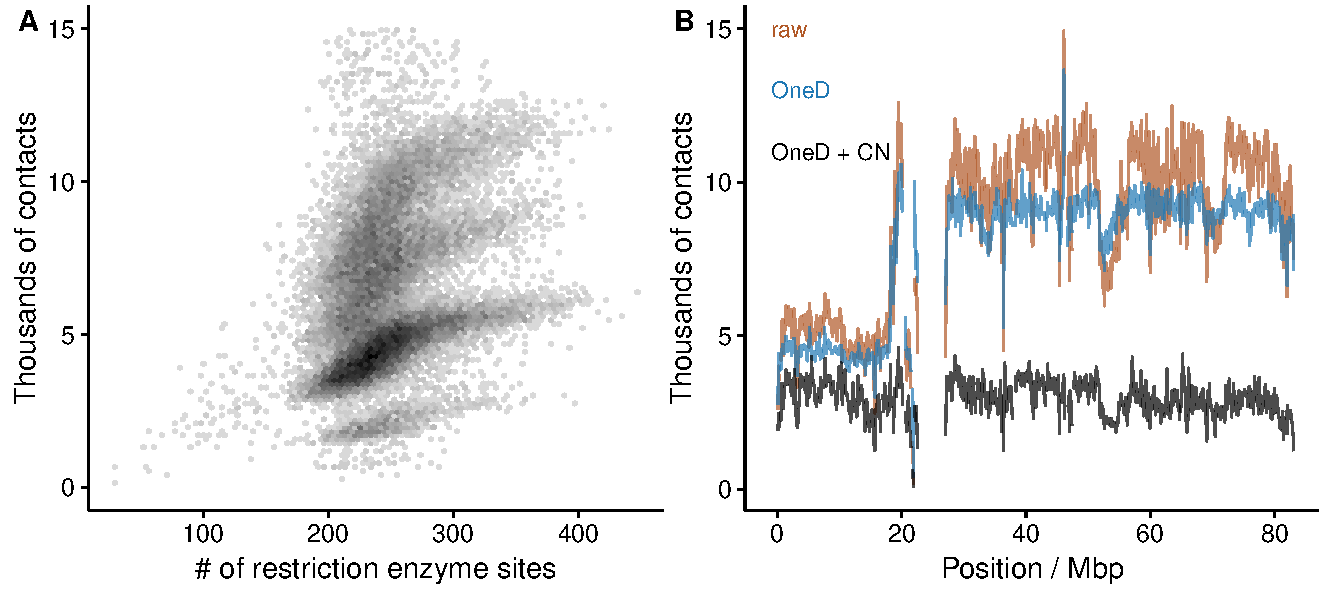
\includegraphics[width=.99\textwidth]{img/figure1.pdf}}
\caption{Total amount of contacts per bin. A. Non linear relationship
between the number of restriction sites and the total number of
contacts per bin in T47D. B. Total number of contacts per bin on
chromosome 17 of T47D. The brown line represents the raw
signal, the blue line represents the signal after bias correction, the
black line represents the signal after bias and copy number (CN) correction.
The long arm of chromosome 17 (the region corresponding to 20-80 Mbp) is
present in four copies, explaining that the signal is about twice higher
than for the short arm.}
\label{fig:totals}
\end{figure}


Experimental biases affect the total amount of contacts in a continuous
but not necessarily linear way. Figure~\ref{fig:totals}A shows the
relationship between the amount of contacts and the number of restriction
enzyme sites in T47D, a breast cancer cell line with an aberrant
karyotype.  Four clouds are visible. Each corresponds to sequences present
in one to four copies. In all of them, the relationship flattens as the
number of restriction sites increases. To capture this
relationship, \textit{OneD} fits a non-linear model between the total
amount of contacts and the known sources of bias (by default the G+C
content, the number of restriction sites and the mappability of the
reads).

The experimental biases are estimated genome-wide and each cell of the
matrix is then corrected using equation (\ref{eq:xhat}). Note that the
corrected amount of contacts is still proportional to the copy number.
Figure~\ref{fig:totals}B shows the corrected number of contacts along
chromosome 17 of T47D. \textit{OneD} greatly reduces the wiggling of the
total amount of contacts (blue line).

% Marc's comment here was regarding lack of motivation and explanation for
% the copy number comparison. I've rescued some text from an older
% version. We should also comment here about CN being a bias or providing
% biological information, so to correct or not to correct for CN

In what follows, we benchmarked \textit{OneD}, against \textit{vanilla},
\textit{ICE} \citep{imakaev2012iterative}, \textit{caICB}
\citep{wu2016computational} and the Local Genomic Features method
\citep[\textit{LGF},][]{hu2012hicnorm, servant2012hitc}. The first three
methods correct biases implicitly, whereas the fourth method does it
explicitly.

Given that our model is based on total number of contacts, we reasoned
that a preliminary test would be to check if the corrected number of
contacts per bin reflects the copy number (as measured by an independent
technique such as array-based copy-number segmentation). We tested the
validity of this approach against the Catalogue Of Somatic Mutations In
Cancer \citep[COSMIC,][]{forbes2010cosmic}. Figure \ref{fig:copy_number}
shows the Pearson correlation between the corrected number of contacts and
the copy number estimation for T47D and K562 (a leukemia cell line with an
aberrant karyotype). Similar results were obtained using Spearman
correlation (Supplementary Figure 1).  All the methods except
\textit{OneD} decreased the agreement between the signal and the copy
number because they partially corrected the discrepancy. In contrast,
\textit{OneD} enhanced the conformity of the signal with the copy number.
Not correcting for variable copy number at that stage may seem
counter-intuitive, but the tests below will show this leads to better
performance.


\begin{figure}
	\centerline{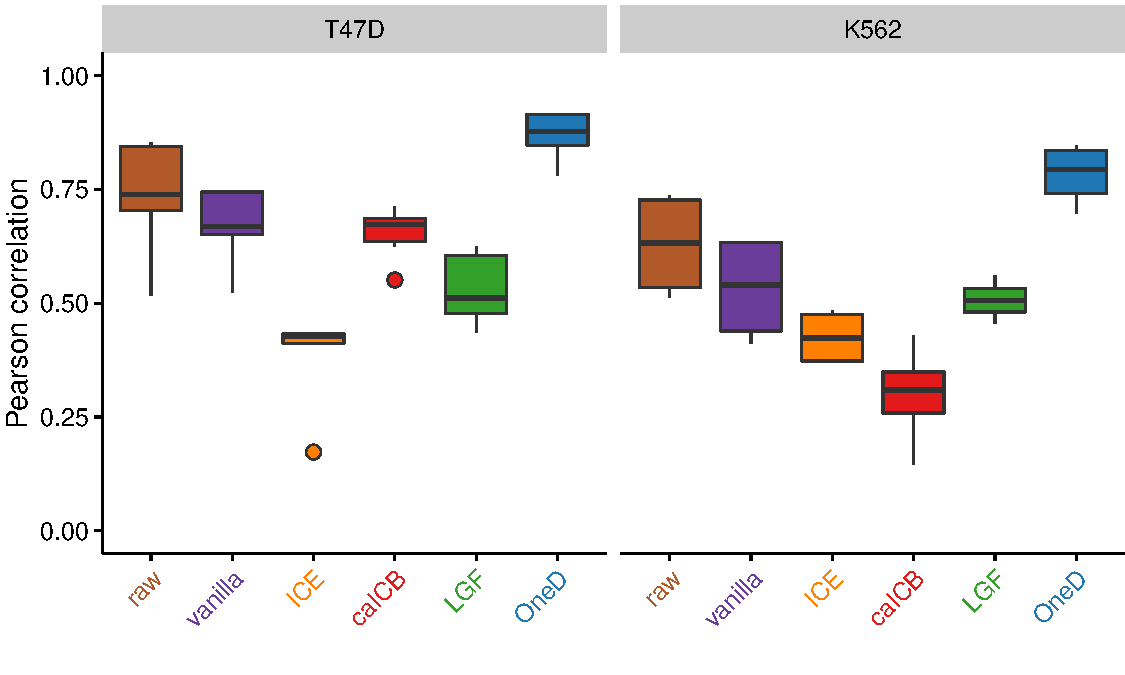
\includegraphics[width=.99\textwidth]
{img/copy_number_figure2.pdf}}
\caption{Pearson correlation between the total number of contacts per bin
and an independent estimation of the copy number (COSMIC). Left panel
T47D breast cancer cell line, right panel K562 leukemia cell line.}
\label{fig:copy_number}
\end{figure}




\subsection{Aberrant karyotypes}

We first benchmarked the performance of our approach on biological
samples with an aberrant karyotype. A good normalization method should
increase the similarity between biological replicates by reducing
irrelevant experimental variance, such as batch effects, laboratory of
origin and protocol variations. Similarly, a good normalization should
decrease the similarity between different samples to enhance the
biological differences.

We assembled two Hi-C data sets obtained from T47D and K562 cells.  In
each set we spiked two samples from the other cell line
(Table~\ref{tab:samples}) to introduce biological variability. We compared
matrices before and after normalization by different methods using the
Pearson correlation of observed over expected counts (see \ref{sec:comp}).
This gave an indication of the impact of a given normalization method. The
results are summarized in Figure~\ref{fig:aberrant}.

The \textit{caICB} and \textit{ICE} methods increased the similarity
between the different cell lines (Figures~\ref{fig:aberrant}A and
\ref{fig:aberrant}B and Supplementary Figures~2 and 3). This is an
undesirable effect, as it obscures the biological variability. Likewise,
these methods decreased the similarity between samples that received the
same treatment (Figure~\ref{fig:aberrant}A), suggesting that the
normalization process is detrimental to the biological signal in these two
cases. The method \textit{vanilla} followed the same trend but to a lesser
extent, consistent with the fact that it consists of a single \textit{ICE}
iteration. \textit{OneD} was the only method to increase the similarity
between experiments carried out on the same material but with a different
protocol (Figure~\ref{fig:aberrant}A).

An important application of normalization methods in experimental setups
is to identify outliers. We thus investigated the capacity of the
different methods to help identify the samples from the other cell type
spiked in the data set. We interpreted the pairwise comparison scores as
classifier scores and summarized the results with a ROC curve
(Figures~\ref{fig:aberrant}C and D). All the methods, including the
absence of normalization, succeeded in identifying the T47D outliers among
the K562 samples, but recognizing the K562 outliers among the T47D samples
proved more challenging. \textit{OneD} increased the discrimination power
compared to the raw matrices, but all the other methods decreased it.
Actually, they performed little better than random on this task. Using the
other metrics described in \ref{sec:comp} yielded similar results
(Supplementary Figures 5, 6 and 7). Note that Spearman correlation of
contacts presented the worst performance for all scenarios, and it thus
seems to be a poor choice for a metric to compare Hi-C matrices.

Taken together, these results show that correcting experimental biases
with \textit{OneD} enhances the biological variation and reduces the noise
on samples with an aberrant karyotype.


\begin{figure}
\centerline{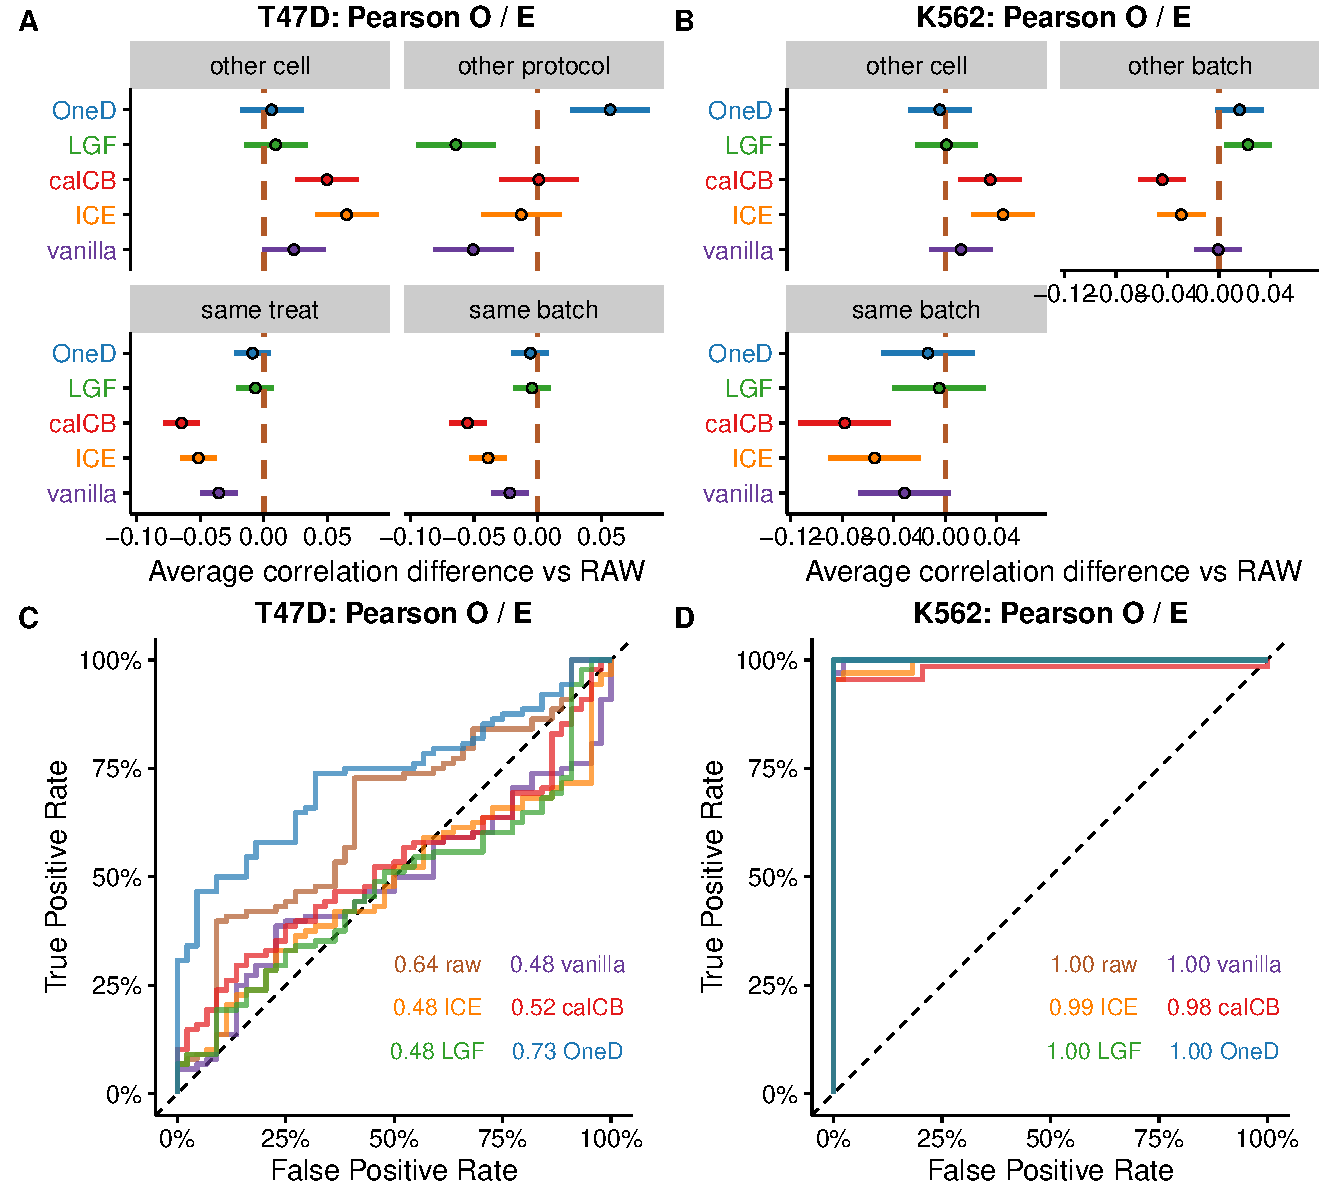
\includegraphics[width=.99\textwidth]
  {img/correlation_aberrant_figure3.pdf}}
\caption{
Results of the comparison between samples with aberrant karyotypes. A and
B. Average changes compared to the raw data on the T47D and K562 sets. The
bars represent 95\% confidence intervals centered on the mean difference
of the correlation score between a given correction method and the raw
data. C and D. ROC curves on the T47D and K562 sets.  The areas under the
curve are indicated in the bottom right corner. The color code is the same
as panels A and B. The brown lines correspond to raw matrices. All results
in this figure are based on Pearson correlations between the observed over
expected counts.}
\label{fig:aberrant}
\end{figure}



\subsection{Normal karyotypes}

Does the performance of \textit{OneD} on aberrant karyotypes come at the
cost of decreased performance on normal karyotypes? To address this
question, we assembled another data set comprised of mouse B cells and
embryonic stem (ES) cells, both with a normal karyotype. The cell types
were pooled in almost equal proportions (see Table~\ref{tab:samples}) and
the same tests as above were performed.

In these conditions, the experimental protocol had a strong effect on the
impact of the different normalization methods (Figure~\ref{fig:normal}A).
For instance, \textit{caICB} and \textit{ICE} increased the similarity
when the protocols were different, but decreased it when the protocols
were the same. The effect was stronger when comparing identical cell
types, but the same trend appeared when comparing different cell types,
indicating that these methods may enhance or reduce biological variation,
depending on the context. Once more, \textit{vanilla} followed the same
trend as \textit{ICE} but to a lesser extent. The \textit{LGF} method
increased the similarity when comparing the same cells with different
experimental protocols, and had little to no effect in the other cases.
This indicates that \textit{LGF} is a safe choice in this case.

\textit{OneD} decreased the similarity between different cell types when
using the same protocol and increased it between identical cell types when
using different protocols. In the other two cases, it had little effect.
In summary, \textit{OneD} never enhanced the experimental noise and even
reduced it in one more case than \textit{LGF}.

When interpreting the similarity scores as classification scores, we
observed that all the methods could identify approximately 50\% of the
biological pairs, after which their performance diverged
(Figure~\ref{fig:normal}B). \textit{OneD} achieved the highest area under
the curve on this problem, but with a small margin over the other methods
except \textit{vanilla}. Using other metrics to compare matrices gave
similar results: \textit{OneD} was always among the top scoring methods
(Supplementary Figures 7 and 8). In these conditions, Spearman correlation
of contacts again appeared as the worst comparison metric because it
showed a lower performance for all the normalization methods.

Taken together, these results indicate that \textit{OneD} performs as well
as the best normalization methods, even with normal karyotypes.

\begin{figure}
\centerline{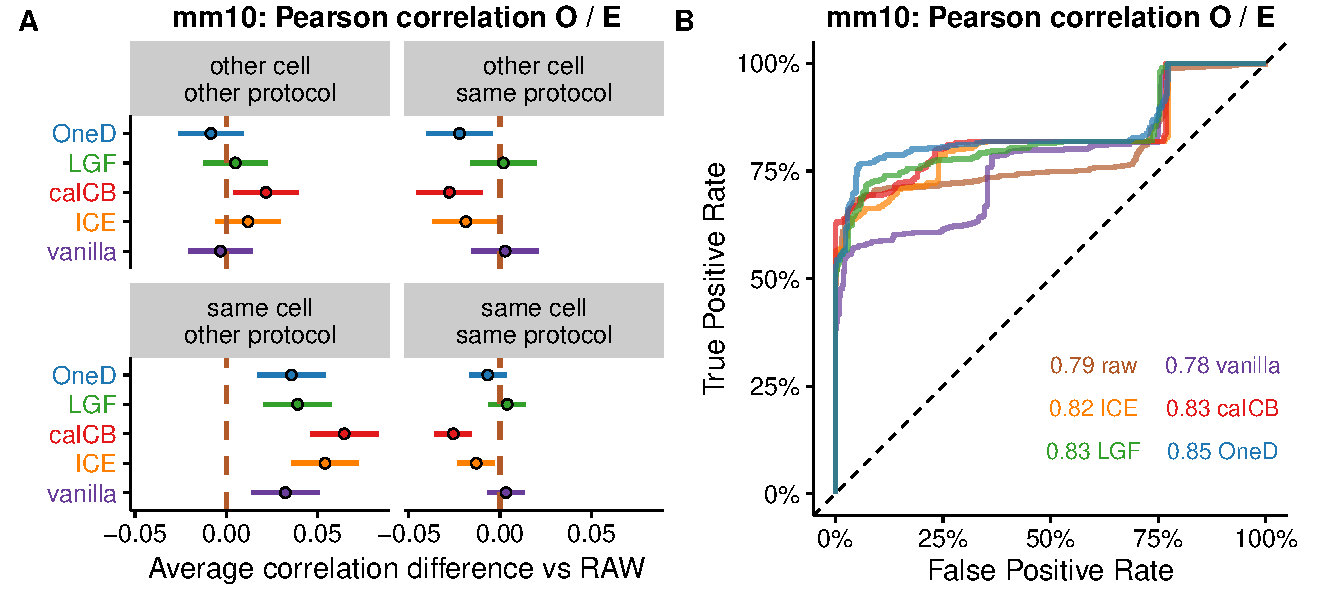
\includegraphics[width=.99\textwidth]
  {img/correlation_normal_figure4.pdf}}
\caption{
Results of the comparison between samples with normal karyotypes. A.
Average changes compared to the raw data on the mouse data set.  B. ROC
curves on the mouse data set. The legend is as in
Figure~\ref{fig:aberrant}.}
\label{fig:normal}
\end{figure}



\subsection{Copy number correction}

Removing the explicit experimental biases enhances the importance of the
copy number in the signal (Figure~\ref{fig:copy_number}). The copy number
is not an experimental bias, but it may be considered an additional source
of bias to be removed. For this reason, \textit{OneD} also allows the user
to correct the copy number and output an euploid-equivalent matrix. To do
so, \textit{OneD} segments the linear signal of the total amount of
contacts into piecewise homogeneous regions. This is carried out by a
hidden Markov model whereby the averages of the states are constrained to
be an integer number, up to a scaling factor (see \ref{sec:hmm}). This
allows the model to detect regions with a number of copies equal to 1, 2,
3 \textit{etc}. With the inferred number of copies at hand, \textit{OneD}
then normalizes each cell of the matrix with equation (\ref{eq:cnvnorm}).

Different normalization methods can either enhance or diminish the signal
in regions with higher copy number (Figure~\ref{fig:cnv_correction}). In
this example, \textit{ICE} overcompensated the original bias at the center
of the picture and faded the signal almost entirely. Concomitantly, the
signal at the bottom left of the matrix was enhanced and showed a
structure that was not visible in the raw data. On the contrary,
\textit{LGF} strengthened the central region and the diagonal.
\textit{OneD} reduced the level of the central portion by a factor 2
approximately, but did not otherwise distort the main features of the
region. This example shows that the copy number does not have a simple and
predictable effect on the final matrix. Not taking it into account may
open the door to some normalization artifacts.

\begin{figure}
\centerline{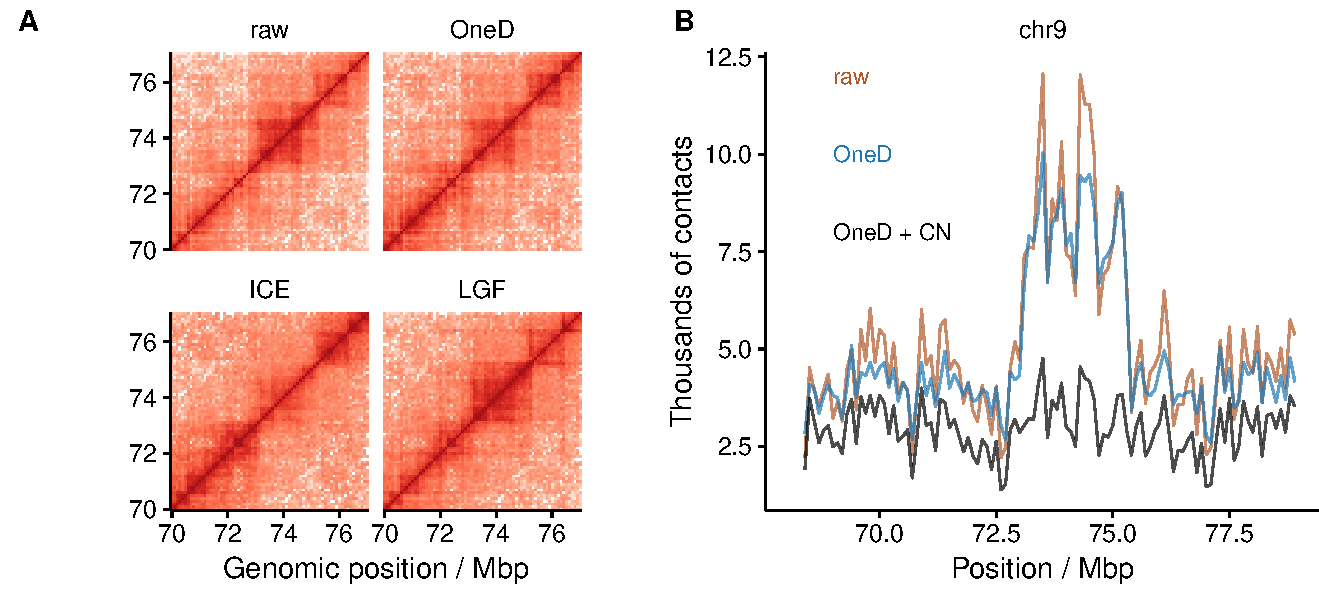
\includegraphics[width=.99\textwidth]
  {img/figure_cnv_correction.pdf}}
\caption{
Copy number correction A. Detail of a Hi-C matrix normalized with
different methods. The central portion has an increased copy number, which
affects normalization. \textit{ICE} fades it away, \textit{LGF} enhances
it and \textit{OneD} reduces the signal by about half. B. Profile of the
total amount of contacts after copy numer correction. The plot shows the
same region as panel A. The brown line represents the raw signal, the blue
line represents the signal after bias correction, the black line
represents the signal after bias and copy number (CN) correction.}
\label{fig:cnv_correction}
\end{figure}

Figure~\ref{fig:cnv_correction}B shows the total sum of contacts after
correction for the copy number with \textit{OneD}. The region around
72.5-75.0 Mbp showed an elevated amount of contacts in the raw data. After
copy number correction, the signal is brought to the same level as the
flanking regions. The result provided by \textit{OneD} is not necessarily
the right one (see Discussion), but at least it does not correct copy
number variations as a side effect of some other criteria.

In summary, \textit{OneD} can be used to obtain an euploid-equivalent
normalized matrix in cases where the effect of the copy number must be
removed from the signal.

\subsection{Speed}

Finally, we compared the computational speed of the different
normalization methods. \textit{vanilla} and \textit{ICE} have broad
acceptance for their conceptual simplicity, ease of use and speed
\citep{imakaev2012iterative}. This is even more significant as current
explicit methods \citep{servant2012hitc} are much slower in comparison.

Unlike the other methods, \textit{OneD} corrects a single variable instead
of the whole matrix, and thus estimates the model parameters much faster
than previous explicit methods. We measured the running time of the
different tools on a 3.3~GHz machine with 62 GB~RAM, always using the
default parameters. Figure~\ref{fig:times}A shows the running times of the
different methods on the samples described in Table~\ref{tab:samples} at
100 kbp resolution. The fastest method was \textit{vanilla} and the
slowest is \textit{LGF}, with an over 100-fold span between the two.

\textit{OneD} was the second fastest method and it always ran in less than
1~min in the conditions of the benchmark. Throughout this benchmark, the
memory footprint of \textit{OneD} was less than 300 MB.  Interestingly,
the running time of \textit{OneD} was much more homogeneous than that of
the other methods. The reason is that the size of the regression problem
to be solved by the \texttt{mgcv} package is always the same at fixed
resolution.

We also performed a benchmark on a smaller data set at increasing
resolution (Figure~\ref{fig:times}B). On this benchmark, \textit{ICE} ran
slightly faster than \textit{OneD}, and the the rank of the methods
remained the same at all resolutions. Taken together, these results show
that \textit{OneD} is competitive in terms of computational speed compared
to existing methods.

\begin{figure}
\centerline{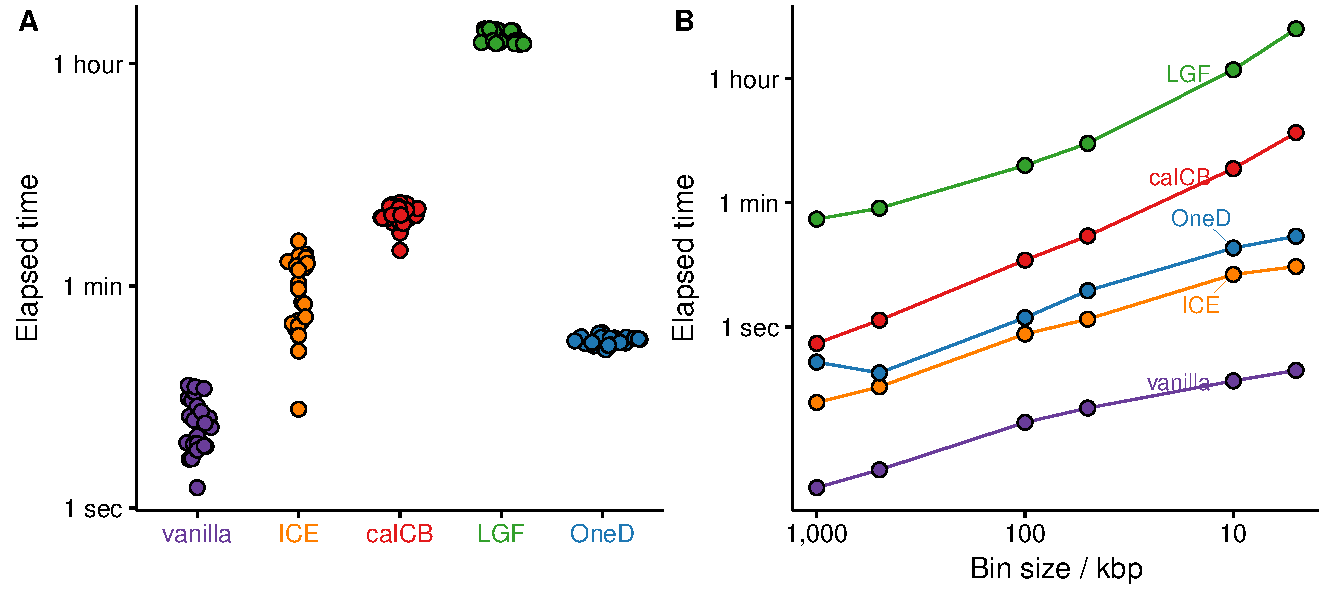
\includegraphics[width=.99\textwidth]
  {img/figure_benchmark_time.pdf}}
\caption{
Computing time of the bias correction methods. A. Total time for the
entire genome at 100 kbp resolution. Each dot corresponds to one sample.
The only method faster than ours under performs in all sample comparisons.
B. Time to correct a reduced genome (chr19-22) of one sample at different
resolutions. Note the logarithmic scale on the y-axis on both panels.}
\label{fig:times}
\end{figure}





%% --------------- Discussion --------------- %%

\section{Discussion and Conclusions}

Here we introduced \textit{OneD}, a fast computational method to normalize
Hi-C matrices. \textit{OneD} was developed ground up to address the need
to normalize data from biological samples with aberrant karyotypes, but it
applies seamlessly to the case of normal karyotypes. We showed that
\textit{OneD} performs significantly better than other methods when the
cells present karyotypic aberrations (Figure~\ref{fig:aberrant}), and that
it performs equally well as the best methods on euploid genomes
(Figure~\ref{fig:normal}). We also showed that \textit{OneD} is
approximately as fast as \textit{ICE}, which makes it competitive from the
point of view of computational speed.

The originality of \textit{OneD} lies in that it projects all the biases
onto a single variable: the total amount of contacts per bin. This allows
greater running speed, while preserving a good performance on samples with
karyotypic aberrations. One of the reasons why \textit{OneD} is able to
better highlight the biological distinctions between samples is that it
only corrects the copy number if specifically requested by the user. The
impact of copy number variations on normalization is rather opaque,
especially if they are treated as implicit biases
(Figure~\ref{fig:cnv_correction}). Treating them as explicit biases with
optional removal seems to be an overall safer strategy.

This raises the question whether variations of the copy number constitute
a biological signal or an artifact. If the biological sample contains
karytoypic aberrations, then its genome is grossly different from the
reference genome, which makes signal correction very challenging. The
proper approach would be to use the actual genome of the biological sample
as a reference to construct the contact map. However, this strategy is
presently unfeasible because assembling mammalian genomes is still a hard
problem.

Depending on the intention of the user, the effect of the copy number
should either be kept or removed. This is why \textit{OneD} does not
perform the correction by default, but allows the user to obtain a
euploid-equivalent Hi-C map computed from a hidden Markov model. The
resulting matrices have a near constant amount of contacts per bin, but
the artifacts caused by the mismatch between the genome of the sample and
the reference genome are still present (for instance, the artifacts caused
by large scale inversions are not changed in any way).

Overall, \textit{OneD} constitutes a novel computational approach to
normalize Hi-C matrices. If the karyotype of the sample is aberrant, it
enhances the biological variation.  If not, it performs at least equally
well as other methods in terms of quality and of computational speed.


\section*{Acknowledgements}

We would like to thank the members of the 4DGenome Synergy project for the
fruitful discussions during project meetings. E.V. wants to acknowledge
the members of Miguel Beato's laboratory for their insights during lab
meetings.

\section*{Author contributions}

Conceptualization, E.V.; Methodology, E.V. and G.F.; Software, E.V. and
G.F.; Formal Analysis, E.V.; Investigation, E.V., F.D., Y.C. and R.S.;
Resources, M.B.; Data curation, J.Q., Writing – Original Draft, E.V. and
G.F., Writing – Review \& Editing, F.D. J.Q., R.S., Y.C, T.G., M.A.M-R.
and M.B.; Visualization, E.V.; Supervision, G.F. and M.B., Project
Administration, M.B.; Funding Acquisition, M.B., T.G., M.A.M-R. and G.F.

\section*{Funding}

This work was partially supported by the Spanish Ministry of Economy and
Competitiveness `Centro de Excelencia Severo Ochoa 2013-2017'
(SEV-2012-0208) and ACER to CRG. R.S. was supported by an EMBO Long-term
Fellowship (ALTF 1201-2014) and a Marie Curie Individual Fellowship
(H2020-MSCA-IF-2014). We received funding from the European Research
Council under the European Union's Seventh Framework Programme
(FP7/2007-2013)/ERC Synergy grant agreement 609989 (4DGenome). The content
of this manuscript reflects only the author's views and the Union is not
liable for any use that may be made of the information contained therein.

\vspace*{-12pt}

\bibliographystyle{natbib}
\bibliography{references}

\end{document}
